%% LyX 2.3.1 created this file.  For more info, see http://www.lyx.org/.
%% Do not edit unless you really know what you are doing.
\documentclass[english]{beamer}
\usepackage{lmodern}
\renewcommand{\sfdefault}{lmss}
\renewcommand{\ttdefault}{lmtt}
\usepackage[T1]{fontenc}
\usepackage[latin9]{inputenc}
\usepackage{amsmath}
\usepackage{amssymb}
\usepackage{graphicx}

\makeatletter
%%%%%%%%%%%%%%%%%%%%%%%%%%%%%% Textclass specific LaTeX commands.
% this default might be overridden by plain title style
\newcommand\makebeamertitle{\frame{\maketitle}}%
% (ERT) argument for the TOC
\AtBeginDocument{%
  \let\origtableofcontents=\tableofcontents
  \def\tableofcontents{\@ifnextchar[{\origtableofcontents}{\gobbletableofcontents}}
  \def\gobbletableofcontents#1{\origtableofcontents}
}

%%%%%%%%%%%%%%%%%%%%%%%%%%%%%% User specified LaTeX commands.
\usetheme{Warsaw}
% or ...

\setbeamercovered{transparent}
% or whatever (possibly just delete it)

\makeatother

\usepackage{babel}
\begin{document}
\title[QCQS]{11-qubit Trapped Ion Quantum Computer and Quantum Simulation with
Trapped Ions}
\author{Quanxin Mei}
\institute{Center for Quantum Information, Institute for Interdisciplinary Information
Sciences, Tsinghua University}
\date{3.22, 2019}

\makebeamertitle

%\pgfdeclareimage[height=0.5cm]{institution-logo}{institution-logo-filename}
%\logo{\pgfuseimage{institution-logo}}

\AtBeginSubsection[]{%
  \frame<beamer>{
    \frametitle{Outline}
    \tableofcontents[currentsection,currentsubsection]
  }
}

%\beamerdefaultoverlayspecification{<+->}
\begin{frame}{Outline}

\tableofcontents{}

\end{frame}

\section{Introduction}

\begin{frame}{Comparison}

\begin{block}<1-2>{Superconducting}
\begin{itemize}
\item IBM Q System One, 20-qubit
\item Google, 72-qubit quantum processor
\item Rigetti, 16-qubit quantum processor
\item \ldots
\end{itemize}
\end{block}
%
\begin{block}<2>{Trapped Ions}
\begin{itemize}
\item IonQ, $160$ qubits storage, performed operations on $79$ qubits,
$13$ two-qubit gates
\item TIQC, to be continued :)
\end{itemize}
\begin{figure}
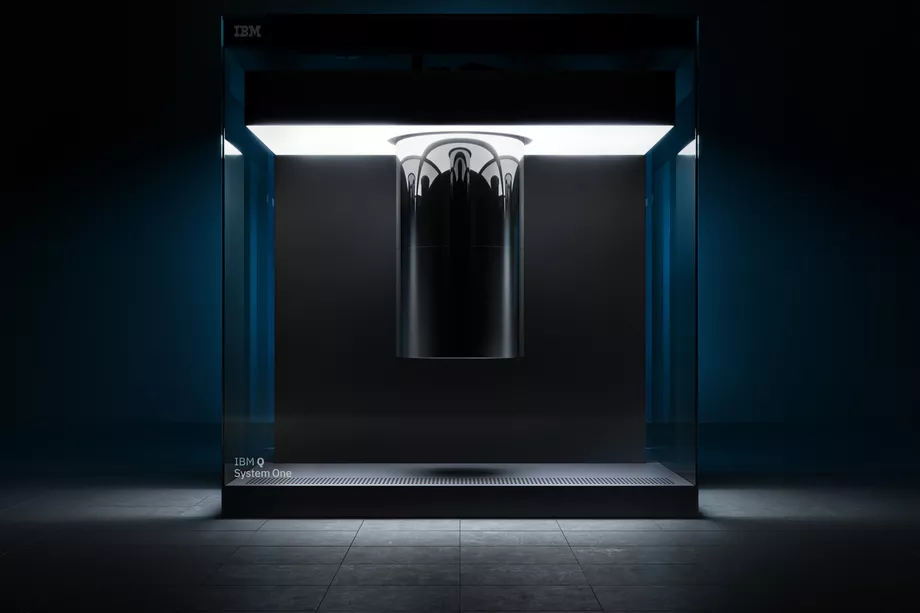
\includegraphics[width=8cm]{ibmq.jpg}

\caption{}

\end{figure}
\end{block}
\end{frame}

\section{IonQ\protect
%
}\begin{frame}{IonQ's 11-qubit Universal Quantum Computer}

\end{frame}

\end{document}
